\chapter*{Dodatak: Prikaz aktivnosti grupe}
		\addcontentsline{toc}{chapter}{Dodatak: Prikaz aktivnosti grupe}
		
		\section*{Dnevnik sastajanja}
		
		
		\begin{packed_enum}
			\item  sastanak
			
			\item[] \begin{packed_item}
				\item Datum: 19. listopada 2023.
				\item Prisustvovali: F. Buhiniček, M. Grdić, M. Sršić, N. Kušen, J. Šarolić, S. Boka, G. Haramija
				\item Teme sastanka:
				\begin{packed_item}
					\item  upoznavanje sudionika 
					\item  dogovaranje prvih koraka
				\end{packed_item}
			\end{packed_item}
			
			\item  sastanak
			\item[] \begin{packed_item}
				\item Datum: 26. listopada 2023.
				\item Prisustvovali: F. Buhiniček, M. Grdić, M. Sršić, N. Kušen, J. Šarolić, S. Boka, G. Haramija
				\item Teme sastanka:
				\begin{packed_item}
					\item  podijelili dijelove dokumentacije članovima za rad (2,3.1,3.1.1 )
					\item  složen osnovni Spring Boot server
				\end{packed_item}
			\end{packed_item}
			
						\item  sastanak
			\item[] \begin{packed_item}
				\item Datum:  2. studenoga 2023.
				\item Prisustvovali: F. Buhiniček, M. Grdić, M. Sršić, N. Kušen, J. Šarolić, S. Boka, G. Haramija
				\item Teme sastanka:
				\begin{packed_item}
					\item  podijelili dijelove dokumentacije (4, 4.1, 4.1.1, 4.1.2, 4.2)
					\item  započeta izrada registracije i login-a (backend, frontend)
				\end{packed_item}
			\end{packed_item}
			
			
									\item  sastanak
			\item[] \begin{packed_item}
				\item Datum: 10. studenoga 2023.
				\item Prisustvovali: F. Buhiniček, M. Grdić, M. Sršić, N. Kušen, J. Šarolić, S. Boka, G. Haramija
				\item Teme sastanka:
				\begin{packed_item}
					\item  pregled napravljenog, dogovor za ispravke, poboljšanja, deploy
				\end{packed_item}
			\end{packed_item}
			
			
			\item  sastanak
			\item[] \begin{packed_item}
				\item Datum: 13. prosinca 2023.
				\item Prisustvovali: F. Buhiniček, M. Grdić, M. Sršić, N. Kušen, J. Šarolić, S. Boka, G. Haramija
				\item Teme sastanka:
				\begin{packed_item}
					\item pregled napravljenog
					\item izrada skica screen-ova
					\item podjela frontend komponenti
				\end{packed_item}
			\end{packed_item}
			
			\item  sastanak
			\item[] \begin{packed_item}
				\item Datum: 22. prosinca 2023.
				\item Prisustvovali: F. Buhiniček, M. Grdić, M. Sršić, N. Kušen, J. Šarolić, S. Boka, G. Haramija
				\item Teme sastanka:
				\begin{packed_item}
					\item  pregled napravljenog
					\item  dogovor o radu za vrijeme praznika
				\end{packed_item}
			\end{packed_item}
			
			\item  sastanak
			\item[] \begin{packed_item}
				\item Datum: 11. siječnja 2024.
				\item Prisustvovali: F. Buhiniček, M. Grdić, M. Sršić, N. Kušen, J. Šarolić, S. Boka, G. Haramija
				\item Teme sastanka:
				\begin{packed_item}
					\item  pregled napravljenog
					\item podjela završnih zadataka
				\end{packed_item}
			\end{packed_item}
			
			\item  sastanak
			\item[] \begin{packed_item}
				\item Datum: 18. siječnja 2024.
				\item Prisustvovali: F. Buhiniček, M. Grdić, M. Sršić, N. Kušen, J. Šarolić, S. Boka, G. Haramija
				\item Teme sastanka:
				\begin{packed_item}
					\item pregled i finalizacija aplikacije i dokumentacije
					\item priprema za predaju
				\end{packed_item}
			\end{packed_item}
			
		\end{packed_enum}
		
		\eject
		\section*{Tablica aktivnosti}
		

			\begin{longtblr}[
					label=none,
				]{
					vlines,hlines,
					width = \textwidth,
					colspec={X[7, l]X[1, c]X[1, c]X[1, c]X[1, c]X[1, c]X[1, c]X[1, c]}, 
					vline{1} = {1}{text=\clap{}},
					hline{1} = {1}{text=\clap{}},
					rowhead = 1,
				} 
			
				\SetCell[c=1]{c}{} & \SetCell[c=1]{c}{\rotatebox{90}{\textbf{Gašpar Haramija}}} & \SetCell[c=1]{c}{\rotatebox{90}{\textbf{Filip Buhiniček}}} &	\SetCell[c=1]{c}{\rotatebox{90}{\textbf{Sandro Boka}}} & \SetCell[c=1]{c}{\rotatebox{90}{\textbf{Marko Sršić }}} &	\SetCell[c=1]{c}{\rotatebox{90}{\textbf{Mateo Grdić}}} & \SetCell[c=1]{c}{\rotatebox{90}{\textbf{Nikola Kušen}}} &	\SetCell[c=1]{c}{\rotatebox{90}{\textbf{Jakov Šarolić }}} \\  
				Upravljanje projektom 		& 40  &  &  &  &  &  & \\ 
				Opis projektnog zadatka 	& 8 & 7 &  &  &  &  & \\ 
				
				Funkcionalni zahtjevi       &  &  &  & 2.5 & 5 &  &  \\ 
				Opis pojedinih obrazaca 	&  &  &  & 18 &  &  &  \\ 
				Dijagram obrazaca 			&  &  & 7 &  &  &  &  \\ 
				Sekvencijski dijagrami 		& 5 &  &  & 1 &  &  &  \\ 
				Opis ostalih zahtjeva 		& 2 &  &  &  &  &  &  \\ 

				Arhitektura i dizajn sustava	 & 3 &  &  & 2 &  &  &  \\ 
				Baza podataka				&  & 9 &  & 1.5 & 10 &  &   \\ 
				Dijagram razreda 			& 2 &  & 6 & 8 &  &  &   \\ 
				Dijagram stanja				&  &  &  & 7 &  &  &  \\ 
				Dijagram aktivnosti 		&  &  &  & 7 &  &  &  \\ 
				Dijagram komponenti			& 7 &  &  &  &  &  &  \\ 
				Korištene tehnologije i alati 		& 7 &5 & 3 & 7 & 5 & 5 & 5 \\ 
				Ispitivanje programskog rješenja 	& 7 & 7 &  &  & 2.5 & 2.5 & 2.5 \\ 
				Dijagram razmještaja			& 7 &  &  &  &  &  &  \\ 
				Upute za puštanje u pogon 		& 6.5 & 1.5 & 1.5 & 1.5 & 1.5 & 1.5 & 1.5 \\  
				Dnevnik sastajanja 			& 3 & 3 &  & 4 &  &  &  \\ 
				Zaključak i budući rad 		& 2 &  &  &  &  &  &  \\  
				Popis literature 			&  &  &  & 1.5 &  &  &  \\  
				Frontend							&  &  & 25 &  & 35 & 40 & 30 \\  
				Backend					& 10 & 37 &  &  & 48 & 40 & \\  
				Deploy					& 15 & 8 &  &  & 8 & 15 &  \\ 
				Opće ažuriranje dokumentacije 	& 10 & 1.5 &  & 17 &  &  &  \\  
				GitHub 							& 10 & 8 &  &  & 5 &  &  \\ 
				Readme, upute							& 2 &  &  & 1 &  &  &  \\  

			\end{longtblr}
					
					
		\eject
		\section*{Dijagrami pregleda promjena}
		
		
		\begin{figure}[H]
			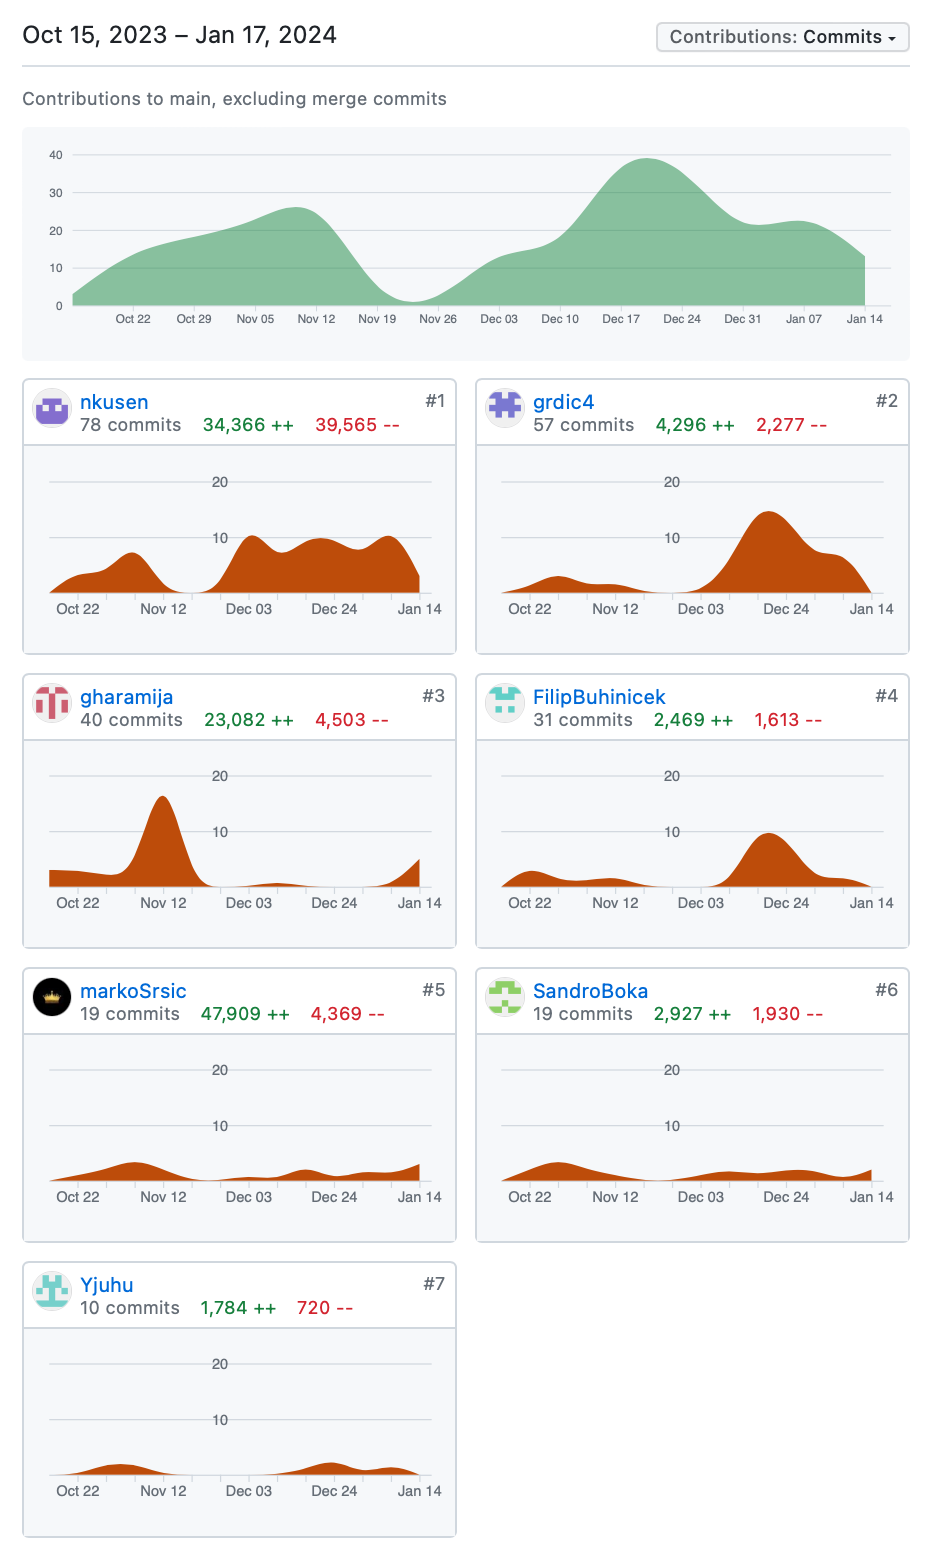
\includegraphics[scale=0.7]{slike/commits.png}
			\centering
			\caption{Dijagram pregleda promjena}
			\label{fig:promjene}
		\end{figure}
	